When a program is compiled to the target architecture, values whose sizes are defined to be smaller than the architectural register size, must be 
adjusted to the register size. This is called sign extension. In C/C++, the use of narrow values remains common for several reasons. Many software systems 
were originally developed for 32-bit architectures
and therefore retained their original data representations, programmers frequently rely on familiar types such as 32-bit `int` even on wider machines, 
and many kinds of data naturally require fewer bits, including characters, and small counters.

LLVM IR provides two bit-extension instructions: sign extension (\texttt{sext}) 
and zero extension (\texttt{zext}). The \texttt{sext} instruction extends the 
bit-width of a value while preserving its sign and numeric value, by replicating 
the most significant (sign) bit into all newly added higher-order bits.
\noindent The \texttt{zext} instruction extends the bit-width of a value by padding all 
newly added higher-order bits with zeros, thus preserving the numeric value mostly
for unsigned integers. 

\begin{center}
  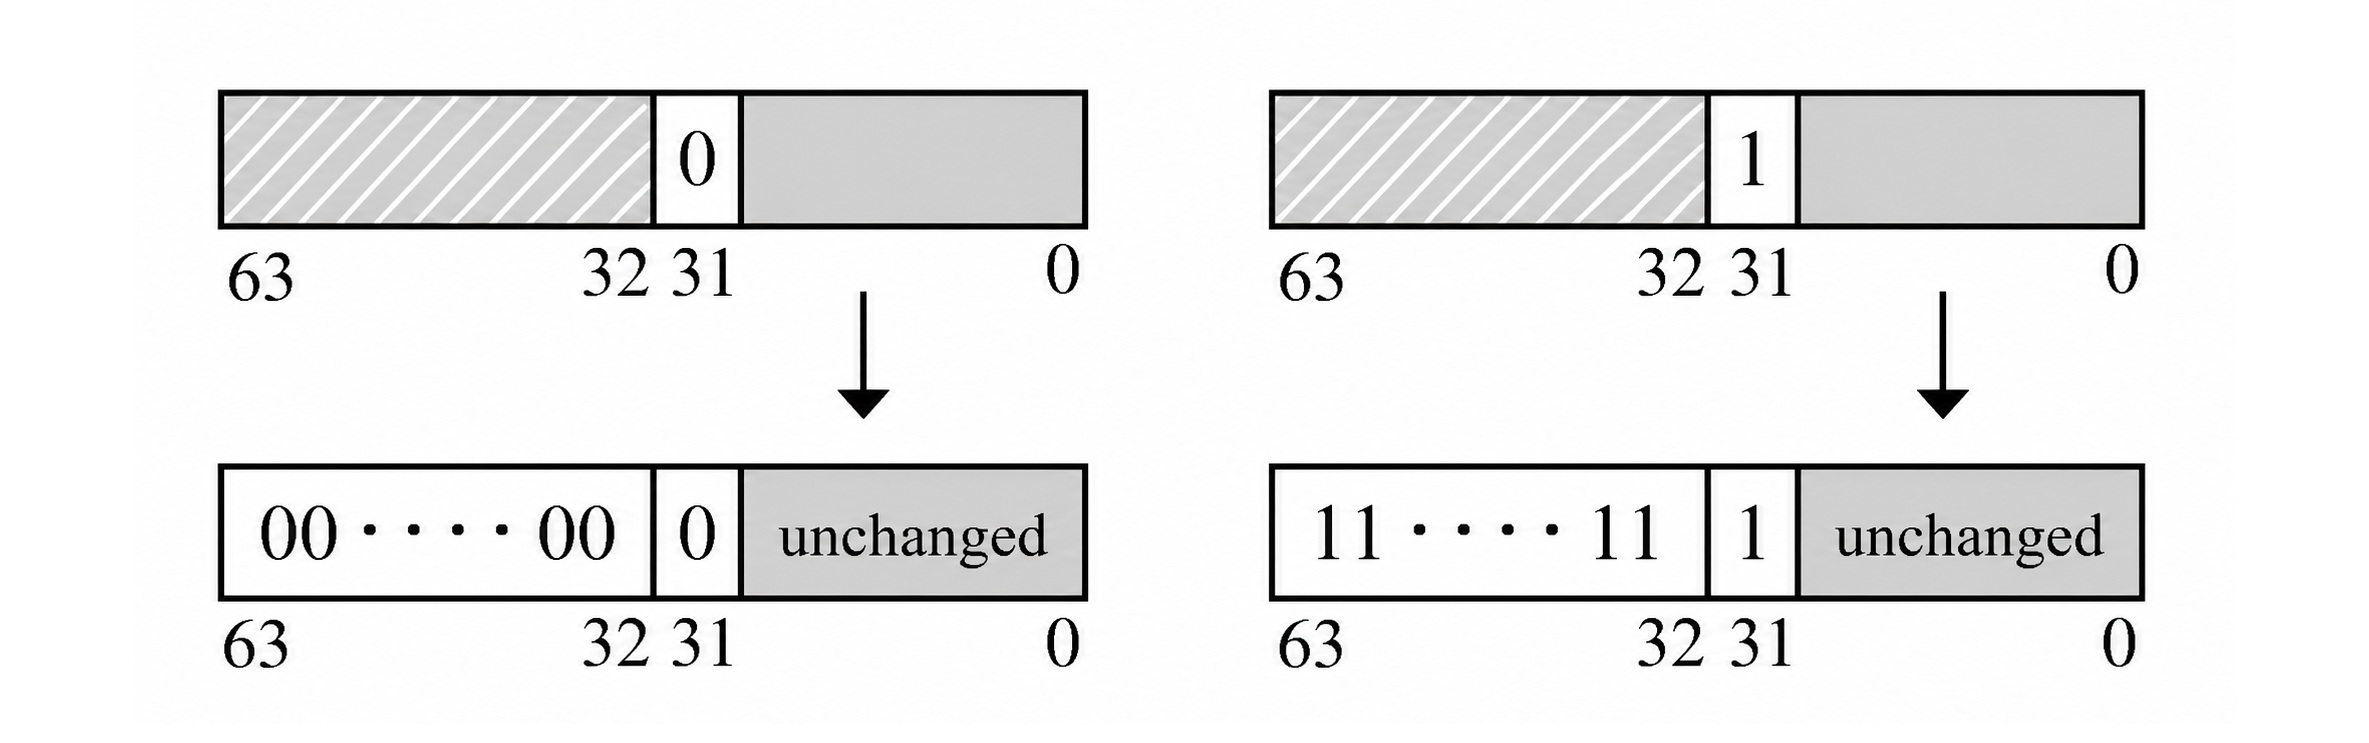
\includegraphics[width=1\columnwidth]{figures/Figure1.jpg}
  \captionsetup{justification=centering,singlelinecheck=false}
  \captionof{figure}{Sign extension of a 32-bit value to a 64-bit value.}
  \label{fig:signext-32-to-64}
\end{center}

\begin{center}
  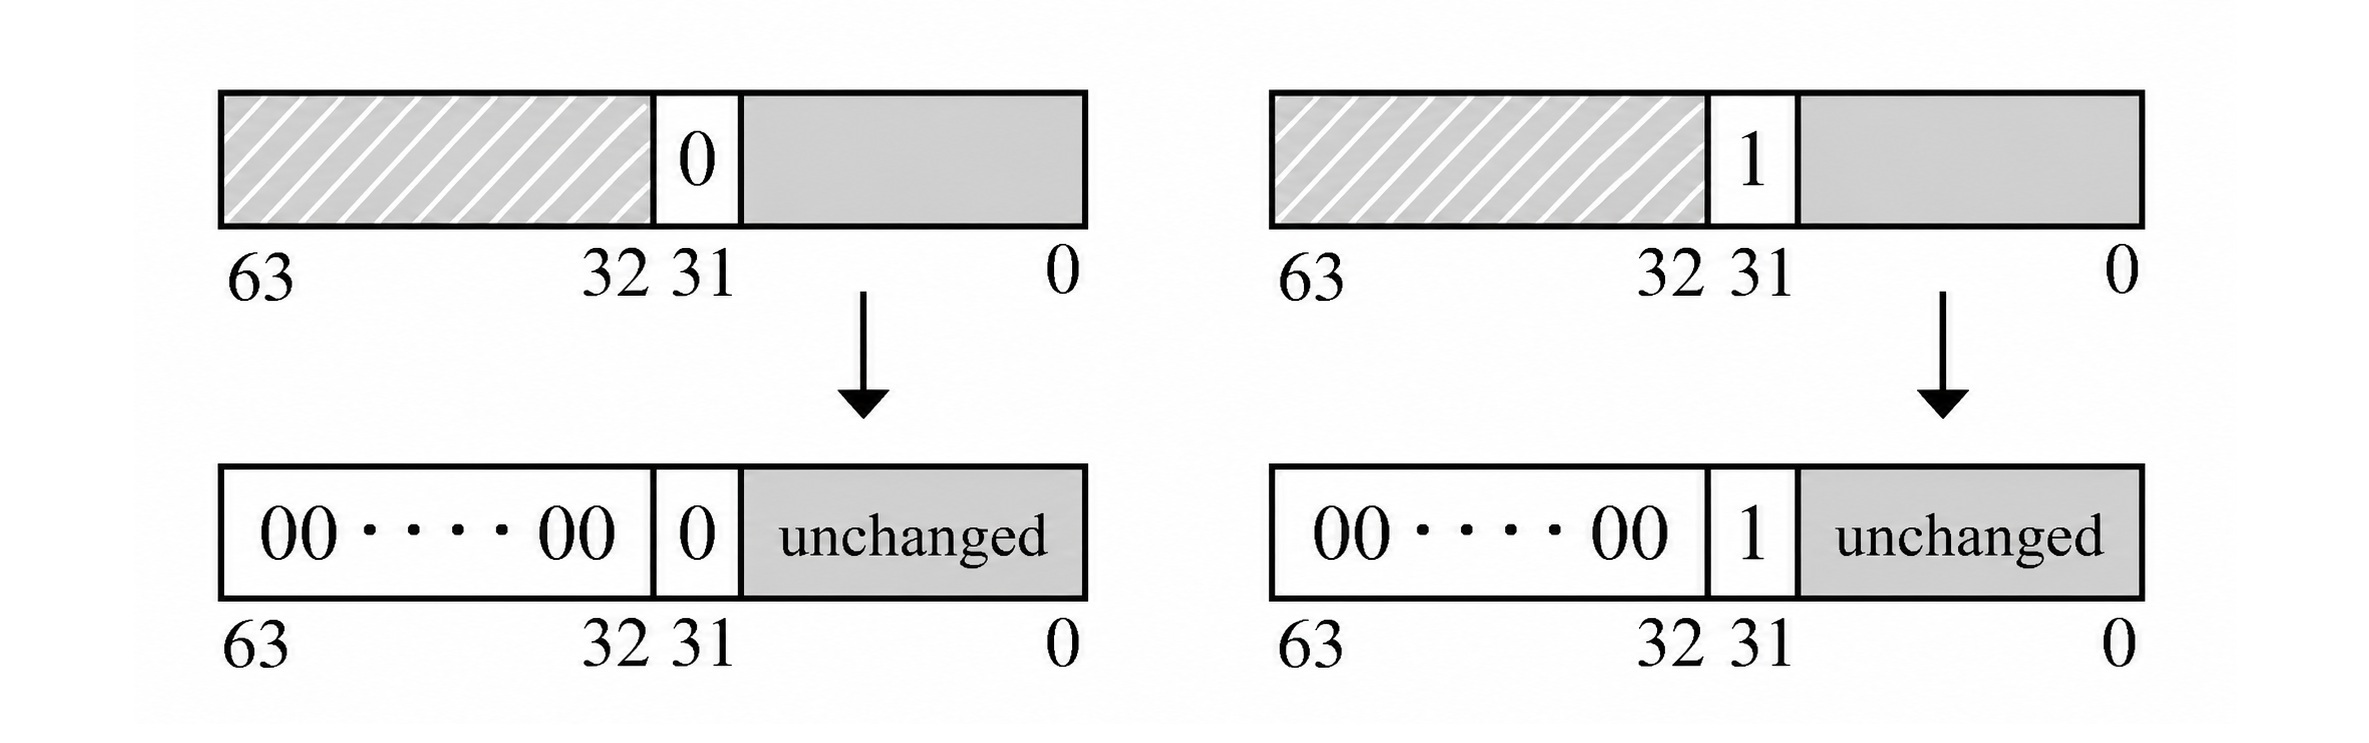
\includegraphics[width=1\columnwidth]{figures/Figure2.jpg}
  \captionsetup{justification=centering,singlelinecheck=false}
  \captionof{figure}{Zero extension of a 32-bit value to a 64-bit value.}
  \label{fig:zext-32-to-64}
\end{center}

In Figures 1 and 2, we see the two basic ways of widening a 32-bit value to 64 bits. Sign extension copies the sign bit into the new upper bits, while zero extension fills the new upper bits with zeros. Although both operations increase the bit-width of a value, they do not always preserve the same meaning. For example, the 32-bit value \texttt{0x80000000} (\texttt{-2147483648}) is negative as a signed 32-bit integer. If it is sign-extended to 64 bits, it becomes \texttt{0xFFFFFFFF80000000} and still represents \texttt{-2147483648}. If the same value is zero-extended instead, it becomes \texttt{0x0000000080000000}, which is interpreted as the positive 64-bit value \texttt{2147483648}. This is why the distinction between sign extension and zero extension becomes important during optimization and code generation.

In most architectures compiled through LLVM, register values are treated as zero-extended by default. As a result, middle-end optimizations 
tend to convert \texttt{sext} instructions into \texttt{zext}, and front-end authors are encouraged to prefer \texttt{zext} over \texttt{sext}. 
This means that by the time we see the IR, many extensions that were originally sign extensions have already been rewritten as zero extensions, 
even when this can no longer be proven from the IR alone. This becomes relevant on RISC-V RV64, where sign extension from 32 to 64 bits is often free, 
while zero extension is not~\cite{karouzakis2025llvm,riscv-isa}.



Motivated by the above, we adapt the algorithm of Kawahito et al.~\cite{kawahito2002effective}, proposed in 2002 for a Java Just-in-Time compiler targeting IA-64, to LLVM's SSA-based IR~\cite{llvm-langref}, targeting RISC-V RV64.
The algorithm inserts extensions at definition points and then selectively eliminates them, starting from the most frequently executed regions of the program. In our implementation, the adaptation is organized around the following main ideas:

\begin{itemize}
\item[--] To test the approach, we implemented two function passes for translating the program to 64-bit and effectively eliminating redundant extension instructions.
\item[--] We evaluated our results using LLVM's test suite and the MiBench benchmarks.
\end{itemize}

